\documentclass{mldsmsc}
% \setlength{\parindent}{20pt}

\title{Probabilistic Matrix Factorisation Algorithms for 12-lead ECG Data}
\author{Joana Levtcheva}
\CID{01252821}
\supervisor{Dr Deniz Akyildiz}
% \date{1 May 2023}
%For today's date, use:
\date{\today}
\logoimg{}


% THIS IS WHERE NEW COMMANDS CAN BE DEFINED
% commands below only used in the proof; otherwise can be deleted
\newcommand{\consta}{a}
\newcommand{\X}{X}
\newcommand{\EE}[1]{ \mathrm{E} [ #1 ] }
\newcommand{\inparenth}[1]{\left( #1 \right)}

\begin{document}

% Generates the Title Page
\maketitle


% Generates plagiarism declaration
\declarationname{Joana Levtcheva}
\declarationdate{\today}
\declaration 

\begin{abstract}
Probabilistic matrix factorisation for high-dimensional time-series data with nonlinear subspace: 12-lead ECG data exploration \newline

\noindent Example: In recent years, matrix factorisation (MF) algorithms have gained popularity in the field of machine learning and have found applications in various fields, such as recommendation systems, image processing and missing data imputation. The MF problem concerns factorising a high dimensional data matrix into two lower dimensional factors. The aim of MF methods is to find the factors such that we have a lower dimensional representation of the data.\newline

\noindent In this thesis, we propose a novel \newline

\noindent The main focus of the research project would be to explore PMF methods applied to high-dimensional time-series data with nonlinear subspace: both considering the time varying component, and treating the whole time series as a batch without considering the time component. More precisely, the project would focus on applying such methods to 12-lead ECG data which is 12-dimensional time-series data with a nonlinear subspace. Some of the tasks which could be explored include: modelling the data so that the future behaviour can be predicted, anomaly detection, imputing missing data, or performing peak detection. \newline

\noindent Using probabilistic methods (and specifically the PMF ones) on ECG data is not widely explored. Applying methods such as Probabilistic Matrix Factorisation (PMF) [1], Probabilistic Sequential Matrix Factorisation (PSMF) [2], Matrix-Variate Gaussian Matrix Factorization (MVGMF) [3], etc. to 12-lead ECG data would showcase novel real-world PMF applications in the medical field, and potentially improve the accuracy and efficiency of ECG data analysis. \newline

\end{abstract}

\begin{acknowledgements}

I would like to...

\end{acknowledgements}

% add glossary?

% table of contents
\tableofcontents

% VERY IMPORTANT
% This command switches from Roman to Arabic numbering for main part of thesis
\mainmatter


\chapter{Introduction}

Matrix factorisation (or also matrix decomposition) in the context of linear algebra is simply a factorisation of a matrix into a product of multiple matrices. Many different decompositions exist, and they find various applications in mathematical problems such as solving systems of linear equations, matrix inversion, determinant computation, eigenvalues problems, solving systems of first order ODEs, etc. \newline

\noindent In this thesis, we are interested in matrix factorisation (MF) in the context of machine learning. Nowadays, MF techniques are highly effective and widely used in unsupervised machine learning. These methods aim to decompose the original matrix into multiple lower-dimensional matrices. By breaking the matrix in these simpler components MF aims to uncover latent structures that are not immediately apparent in the original matrix. Some applications are in image processing: for reducing dimensionality and noise in images, NLP for topic modelling, missing data imputation, recommendation systems, etc. \newline

\noindent Formally, we are interested in the general problem of factorising a data matrix $Y \in \mathbb{R}^{m \times n}$ as

\begin{equation}
Y \approx CX,
\end{equation} \newline
\noindent where $C \in \mathbb{R}^{m \times r}$ is the \textit{dictionary matrix}, $X \in \mathbb{R}^{r \times n}$ is the \textit{coefficients matrix} (with columns the coefficients), and $r$ is the \textit{approximation rank} (\cite{cite-key}). Visually we can present the problem as

\begin{equation}
\underbrace{
\begin{bmatrix}
  \times & \times & \times & \times & \times \\
  \times & \times & \times & \times & \times \\
  \times & \times & \times & \times & \times
\end{bmatrix}
}_{\text{Y $\in \mathbb{R}^{m \times n}$ }}
\approx
\underbrace{
\begin{bmatrix}
  \times & \times \\
  \times & \times \\
  \times & \times
\end{bmatrix}
}_{\text{C $\in \mathbb{R}^{m \times r}$ }}
\underbrace{
\begin{bmatrix}
  \times & \times & \times & \times & \times \\
  \times & \times & \times & \times & \times
\end{bmatrix}
}_{\text{X $\in \mathbb{R}^{r \times n}$ }}.
\end{equation}

\noindent There are also probabilistic versions of MF which incorporate probabilistic models to better handle uncertainty and variability in the data, leading to more accurate predictions. Such methodologies postulate a prior distribution over the latent factors and necessitate the computation of the posterior distribution to derive updated estimates. With that the matrix is not only decomposed but probabilistic interpretations of the factors are also possible. Despite considerable progression in the probabilistic versions, there is demand for such methods in applications such as uncertainty quantification, managing time-series data, and executing efficient probabilistic components. \newline

\noindent We should also note that some algorithms are suitable for sequential data - updating $C$ and $X$ incrementally as new data points are observed and thus incorporating temporal dynamics and sequential dependencies into the factorisation process, and others are non-sequential - treating the dataset as a batch independent of the time varying component. \newline

\noindent Throughout this thesis we are going to focus on probabilistic MF algorithms, along with their application to 12-lead ECG data, targeting the problem of managing high-dimensional time-series data. Some examples of such probabilistic MF algorithms are Probabilistic Matrix Factorisation (PMF) (\cite{NIPS2007_d7322ed7}), Dictionary filtering (\cite{cite-key}), Probabilistic Sequential Matrix Factorization (PSMF) (\cite{akyildiz2021probabilistic}), MLE-SMF?. \newline

\noindent The paper "Probabilistic matrix factorisation" (PMF) (\cite{NIPS2007_d7322ed7}) introduces an efficient and scalable probabilistic model for collaborative filtering. The algorithm performs well on large, sparse and imbalanced datasets. This is demonstrated by using a Netflix dataset, where PMF models the user preference matrix $R$ as a product of two lower-dimensional matrices: user feature matrix $U$ and movie feature matrix $V$. The conditional distribution over observed ratings is modeled using Gaussian noise, and zero-mean spherical Gaussian priors are placed on the user and movie feature vectors. The paper also presents two extensions to the initial PMF model: incorporating \textit{adaptive priors} to automatically control the model complexity through these priors over the model parameters, and a \textit{constrained PMF} version to handle and improve predictions for users with few ratings by incorporating constraints based on the assumption that users with similar movie ratings have similar preferences. The authors show that PMF significantly outperforms traditional Singular Value Decomposition (SVD) (\cite{4ba978eb-d878-342d-a11e-6d7554474b2d}) models and scales linearly with the number of observations. It's worth noting that PMF treats each rating as an independent event meaning the time varying component is not taken into consideration, making PMF a batch learning model designed to process large datasets in a non-sequential manner. \newline

\noindent In the paper "Dictionary Filtering: A Probabilistic Approach to Online Matrix Factorization" (\cite{cite-key}), the authors introduce a novel online MF algorithm known as dictionary filtering. It leverages probabilistic models, specifically using recursive linear filters, and efficiently factorises the original data matrix into a dictionary matrix and a coefficients matrix. This is an online and sequential algorithm, meaning it is suitable for high-dimensional and time-varying data, and it also has easy to tune parameters. Although the model can learn nonstationary and dynamic data, it is developed for linear and Gaussian state space models (SSM). 

(Particularly for ECG data, ECG has a nonlinear SSM which doesn't suit the dictionary filtering.) -> Efficient for high-dimensional data, adaptable to non-stationary environments, removes the need for step-size tuning; flexible and computationally efficient: $O(mr^2)$ independent of the number of data points. \newline

\noindent Later, Akyildiz et.al. develop Probabilistic Sequential Matrix Factorization (PSMF) (\cite{akyildiz2021probabilistic}). This method is tailored to time-varying and non-stationary datasets consisting of high-dimensional time-series. Nonlinear Gaussian SSM are considered, decomposing the original matrix into a dictionary matrix and time-variying coefficient matrix. This time, the matrices are with potentially nonlinear dependencies. The model is demonstrated to work on tasks such as forecasting, changepoint detection, missing data imputation, and is shown to work on real-world data with a periodic subspace. There is also a robust version using Student-t filters to handle model misspecification.

PSMF efficiently captures temporal dependencies through Markovian structures on the coefficients, making it possible to encode the dependencies into a lower dimensional latent space. Strengths: Handles non-stationary and time-varying data, robust to model misspecification, efficient sequen- tial inference. Suitable for: modelling data with periodic subpaces, high-dimensional data by reducing it to lower-dimensional latent space, data imputation,
Weaknesses: Potential problems with very large datasets, having many data points. \newline

\noindent In the unpublished MSc thesis (Imperial College London) of Rina Maletta (\cite{rina}), the author introduces Matrix-Variate Gaussian Matrix Factorization (MVGMF). This is a novel PMF method using matrix-variate Gaussian distributions. The algorithm has fast Gaussian updates which take the form of a preconditioned MF algorithm which is stable. An extension for handling missing data and data imputation is also proposed. The method is tested on the Netflix Prize dataset, London air quality (NO2) data, and Olivetti face image dataset.

\section{Contributions}

We outline the contributions made in this thesis. In this thesis, we 

introduce
a novel approach to the MF problem, by proposing a Matrix-Variate Gaussian Matrix
Factorisation (MVGMF) algorithm.

\begin{itemize}
  \item Apply PSMF to 12-lead ECG data -> not applied to such data before
  \item Fourier basis and higher rank (bug in the original code) -> not applied before
  \item Forecast, data imputation, R-peaks
\end{itemize}

The main focus of the research project would be to explore PMF methods applied to high-dimensional time-series data with nonlinear subspace: both considering the time varying component, and treating the whole time series as a batch without considering the time component. More precisely, the project would focus on applying such methods to 12-lead ECG data which is 12-dimensional time-series data with a nonlinear subspace. Some of the tasks which could be explored include: modelling the data so that the future behaviour can be predicted, anomaly detection, imputing missing data, or performing peak detection. \newline

\noindent Using probabilistic methods (and specifically the PMF ones) on ECG data is not widely explored. Applying methods such as Probabilistic Matrix Factorisation (PMF) [1], Probabilistic Sequential Matrix Factorisation (PSMF) [2], Matrix-Variate Gaussian Matrix Factorization (MVGMF) [3], etc. to 12-lead ECG data would showcase novel real-world PMF applications in the medical field, and potentially improve the accuracy and efficiency of ECG data analysis. \newline

PSMF applied to 12-lead ECG data -> imputation, forecasting, R peaks detection \\

Multiple Fourier terms, higher rank for this case (check the paper) \\

\section{Notation}


Throughout this thesis, we will denote the data matrix with $Y$, and the factors as $C$
and $X$. We denote the vectorised forms of the matrices with their respective lower case letters. We can formally define c = vec(C), where vec(·) is the vectorisation operation. The columns of C are stacked on each other, so if C ∈ Rm×r, then c ∈ Rmr×1. We can
also define the inverse vectorisation operator C = vec−1(c). \newline

\noindent We have that p(x) denotes the probability density function (pdf) of x and p(y|x) is the
conditional density of y given x. Where A ∈ Rm×n is a matrix, then MN(A;M,U, V )
denotes the matrix normal pdf for A, where M ∈ Rm×n is the mean, U ∈ Rn×n is the
among-row co-variance and V ∈ Rm×m is the among-column co-variance. We also define
the multivariate normal distribution in the following way; let a ∈ Rm, then N(a; μ, Σ)
denotes the pdf of the multivariate normal distribution for the random variable a, where
μ ∈ Rm is the mean and Σ ∈ Rm×m is the covariance matrix. Im ∈ Rm×m is the m×m
identity matrix. \newline

\noindent Mathematics notation $f_{\theta}$

\chapter{Background}

Background chapter.

\section{Preliminaries}

\section{PMF}

In this section, we will outline the Probabilistic Matrix Factorisation (PMF) algorithm.
This MF technique was proposed by Mnih and Salakhutdinov (2007). PMF is also concerned with factorising a data matrix, not necessarily non-negative,
Y ∈ Rm×n into two lower dimensional matrix factors C ∈ Rm×r and X ∈ Rr×n. However,
unlike NMF, PMF adopts a probabilistic framework. In the PMF case, the matrix
C contains the basis vectors, and X contains the co-efficients. The linear combination
of these reconstruct the data matrix Y . The best reconstruction is determined by the
rank-approximation, r. The exact inference of the probabilistic models proposed by
Hofmann (1999) and Marlin (2003), which make the connection between unobserved
latent features and the observed features, is intractable. The PMF technique is useful
in settings where the data set we are working with is sparse, large and imbalanced.
The method was applied to the Netflix Prize dataset (Bennett et al., 2007), it contains
ratings from 480, 189 users, for 17, 770 movies, with over 100 million observations. The
pre-processing of this dataset consists of creating an m × n ratings matrix, where m is
the number of users, and n is the number of movies, so the i, jth element of the matrix
is user i′s rating of movie j. The ratings are numbered from 1 to 5, with missing ratings
indicated by 0. Since it is not expected that every user rates every movie, the dataset
is very sparse and also imbalanced, since users have different frequencies of rating movies.
In the context of the Netflix Prize dataset, our formulation Y ≈ CX becomes, Y is the
ratings matrix with m users and n movies, C is the latent user matrix and X is the
movie feature matrix.

Model 

Algorithm

\section{DF}

Section content goes here.

\section{PSMF}

Section content goes here.

\subsection{rPSMF}

Some text

\section{NMF}

Section content goes here.

\section{MVGMF}

Section content goes here.

\section{MLE-SMF}

Check this

\section{ECG/medical introduction}

A 12-Lead ECG (Electrocardiogram) is a standard diagnostic tool used to assess the electrical activity of the heart. It provides a comprehensive view of the heart's electrical activity from different angles. The 12 leads consist of:

\begin{itemize}
  \item 6 precordial leads (V1-V6) placed on the chest
  \item 3 limb leads (I, II, III)
  \item 3 augmented limb leads (aVR, aVL, aVF)
\end{itemize}

Each lead records the heart's electrical activity from a different perspective, providing information on:

\begin{itemize}
  \item Heart rate and rhythm
  \item Conduction abnormalities
  \item Chamber enlargement
  \item Myocardial ischemia or infarction
  \item Electrolyte imbalances
\end{itemize}

The ECG machine typically records data for about 10 seconds, producing a graph of voltage versus time.

There are 10 physical electrodes placed on the patient's body. Despite having only 10 electrodes as seen in \ref{fig:combined}, the system provides 12 different "views" or "leads" of the heart's electrical activity. This is achieved through:

\begin{itemize}
    \item 6 precordial leads (V1-V6): These come directly from 6 of the electrodes on the chest.
    \item 3 limb leads (I, II, III): These are derived from electrodes placed on the limbs.
    \item 3 augmented limb leads (aVR, aVL, aVF): These are calculated mathematically from the limb electrodes.
\end{itemize}

So while there are 10 physical connection points, the ECG machine uses these to generate 12 different perspectives or "leads" of the heart's electrical activity.

\hline

The Electrocardiogram (ECG) is a crucial diagnostic tool in cardiology that records the electrical activity of the heart. A standard 12-lead ECG system provides multiple perspectives of cardiac electrical activity, facilitating comprehensive analysis.
Key points for a mathematical focus:

Signal Acquisition: ECG data is acquired through electrodes placed on the body surface, measuring potential differences over time.
Waveform Components: The ECG waveform consists of P, Q, R, S, and T waves, each representing specific cardiac events.
Lead System: The 12-lead system comprises:

6 precordial leads (V1-V6)
3 limb leads (I, II, III)
3 augmented limb leads (aVR, aVL, aVF)

add images sources

\begin{figure}[h!]
    \centering
    \subfigure{
        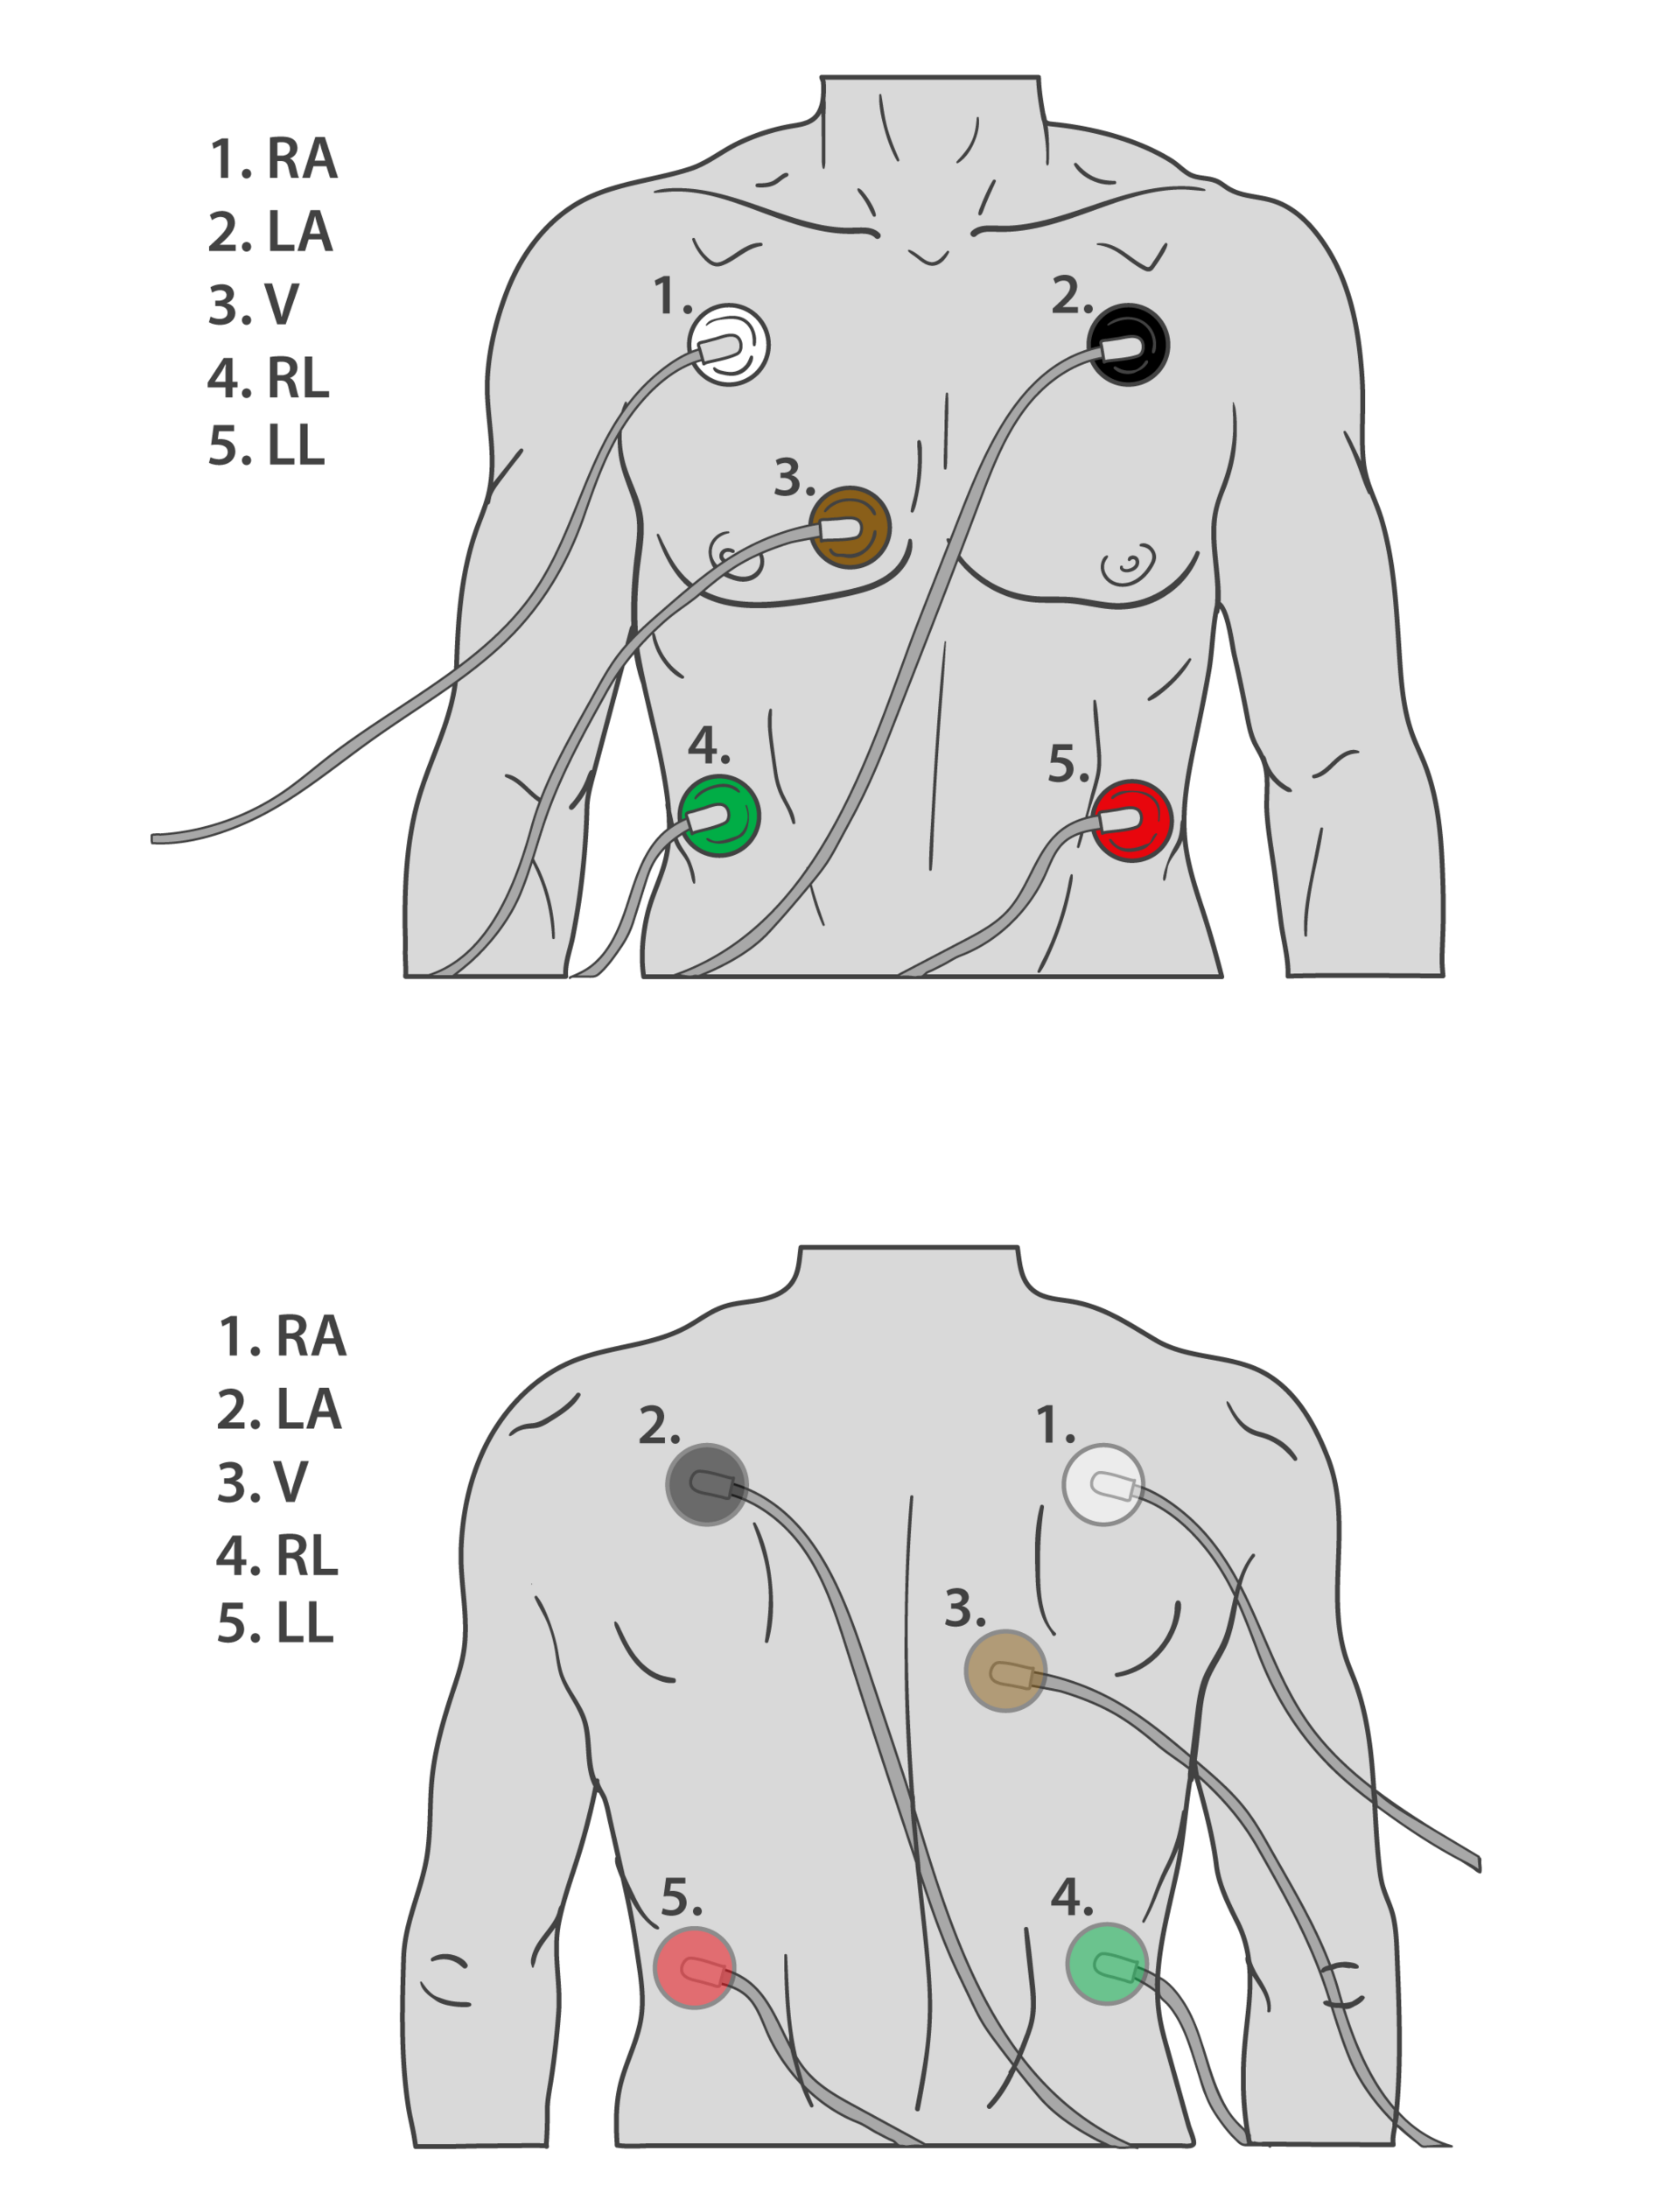
\includegraphics[width=0.48\linewidth]{images/ECG_Electrode_Placement.png}
        \label{fig:ecg-electrode}
    }
    \hfill
    \subfigure{
        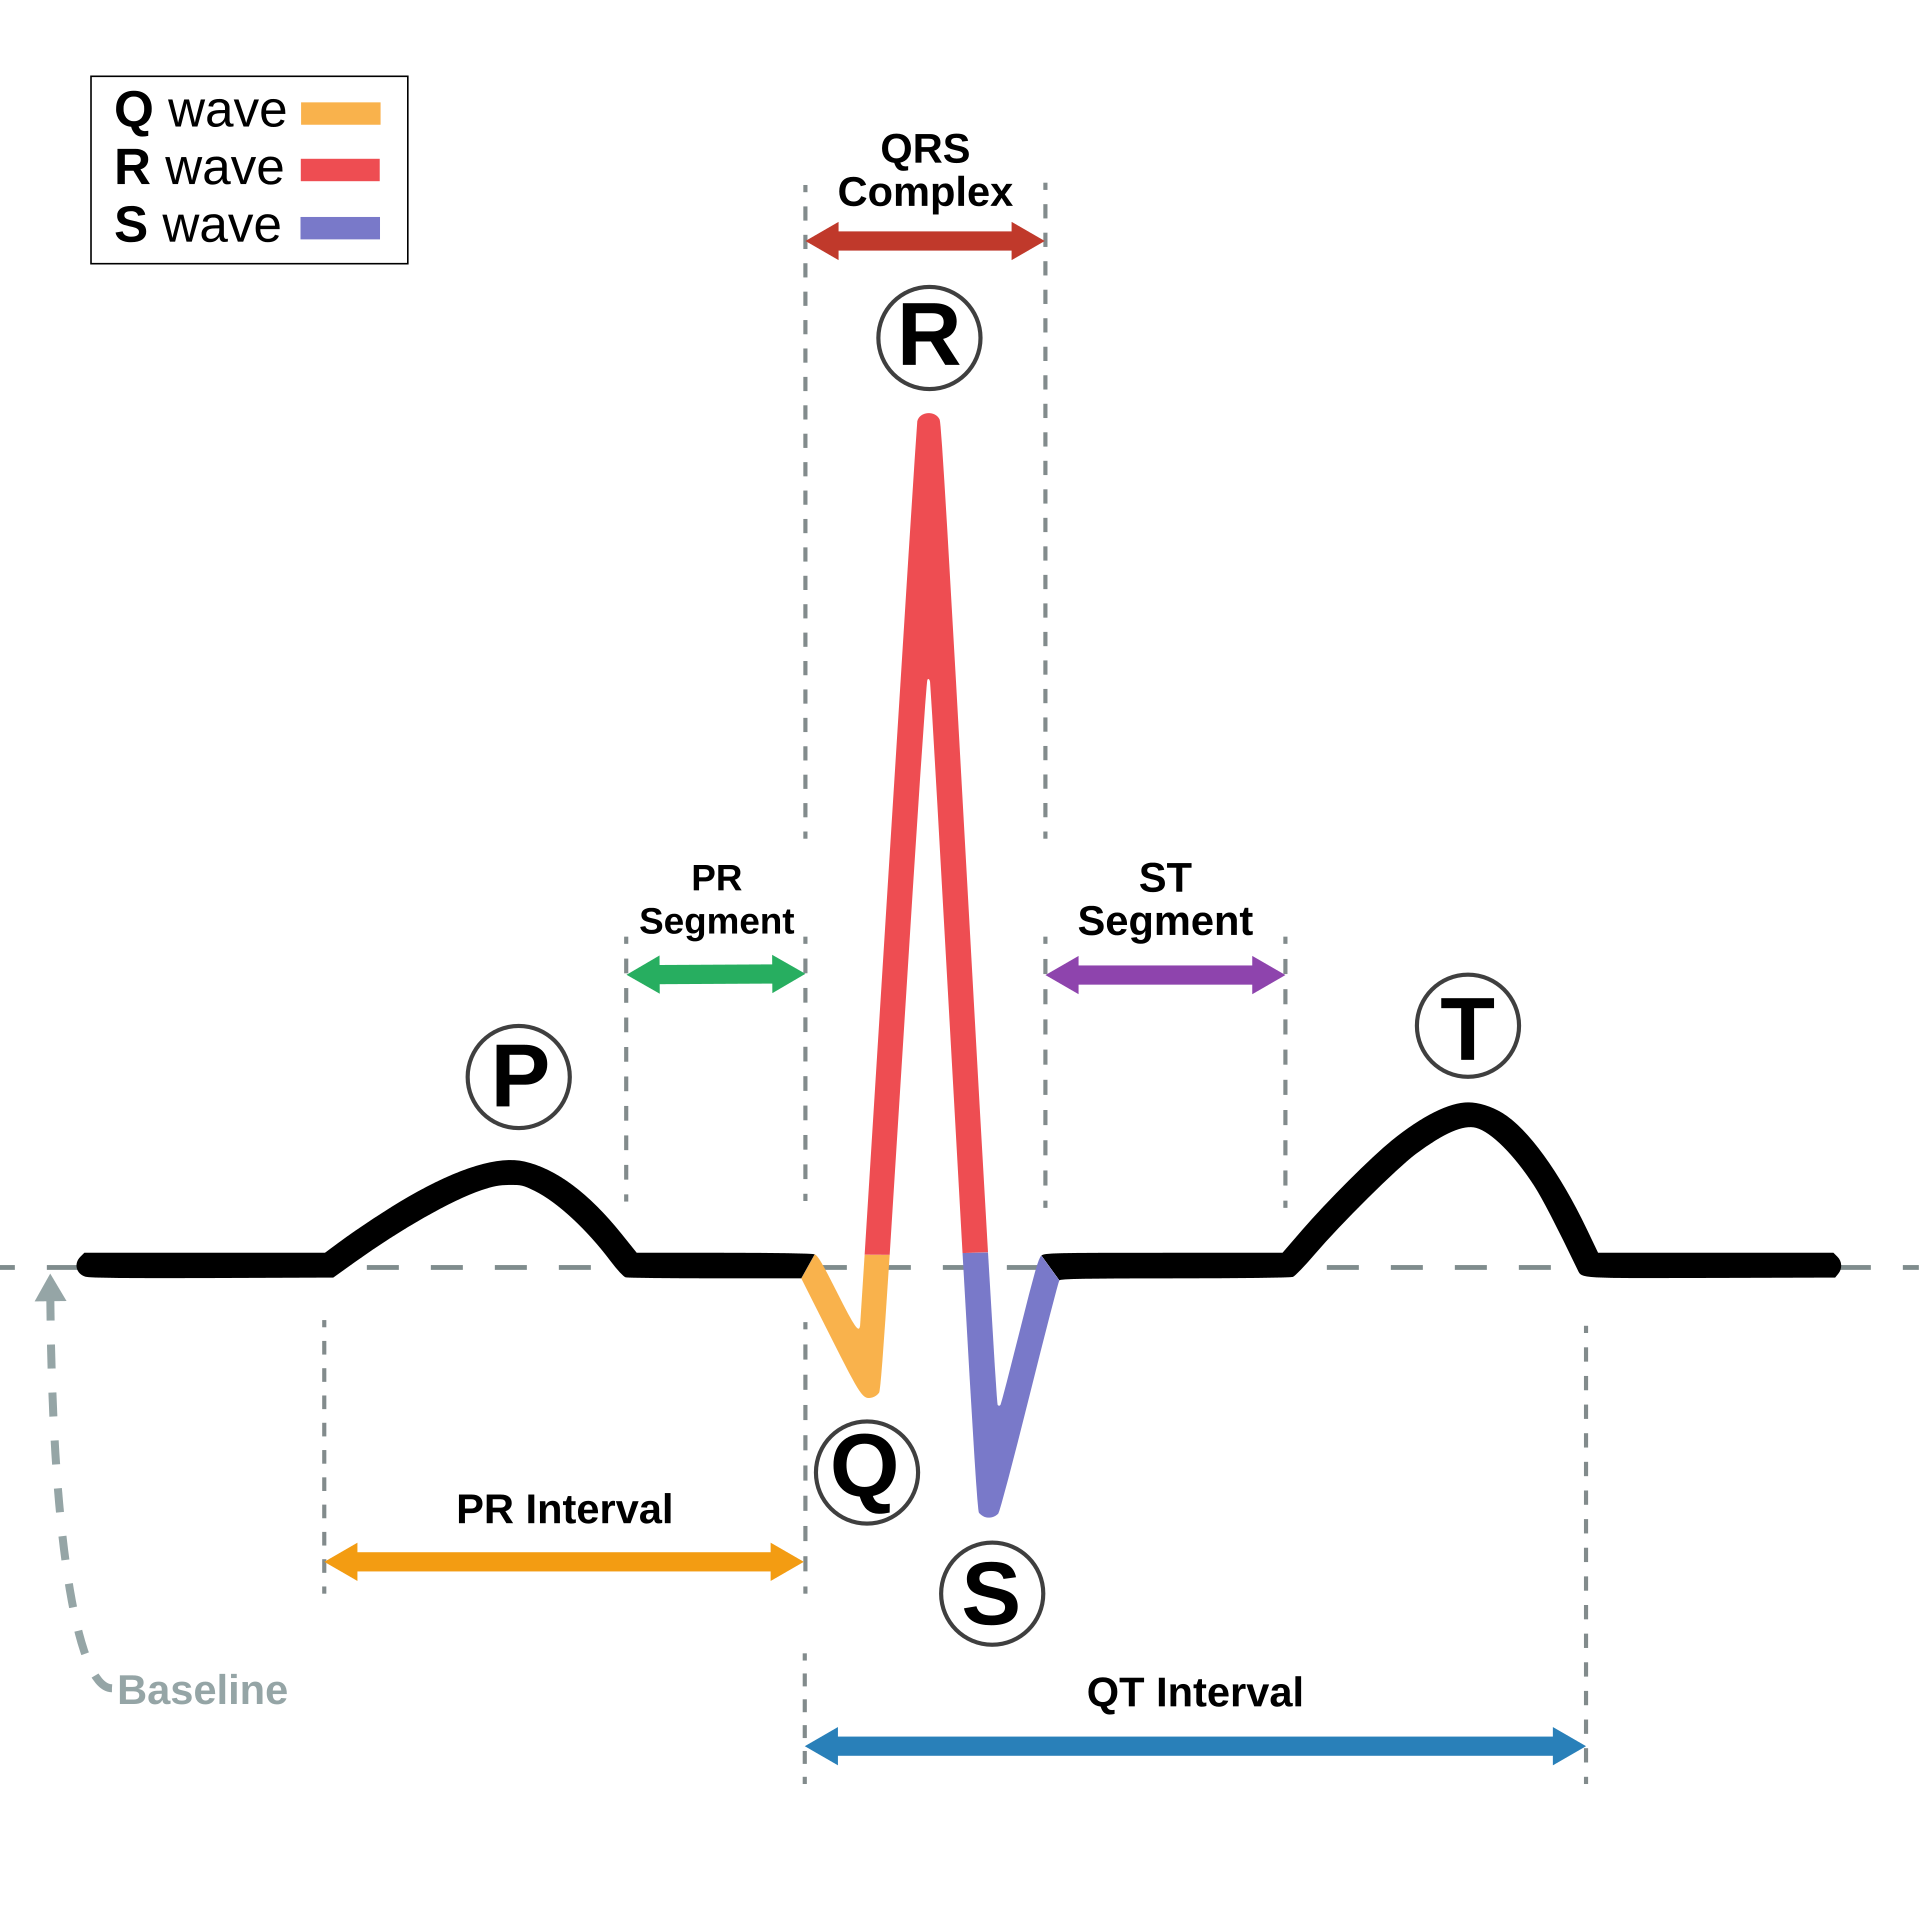
\includegraphics[width=0.48\linewidth]{images/SinusRhythmLabels.png}
        \label{fig:sinus-rhythm}
    }
    \caption{Left: . Right: }
    \label{fig:combined}
\end{figure}

PQRST complex, R-peak..., diagram, data 

% forcing a page break
\clearpage

\chapter{PSMF/etc for ECG}

Describe algorithm \\

Focus on the application to ECG data -> challenges, characteristics, data pre, post, processing 

\chapter{Experiemnts and Results}

Add citations 

The research aims to use the already available A Large Scale 12-lead Electrocardiogram Database for Arrhythmia Study [5], [6], [7]. This is a comprehensive database of high-quality 12-lead ECG signals collected from 45,152 patients. Each signal is with length of 10 seconds corresponding to 5000 data points. The dataset is designed to support arrhythmia research, containing labeled data for various cardiac conditions such as atrial fibrillation, premature ventricular contractions, and bundle branch blocks. This large dataset has high-quality labels from professional experts, diverse arrhythmia types, and additional cardiovascular conditions, making it suitable for performing different research tasks on it without spending time on gathering, cleaning and processing data. \newline


• Presents a comprehensive database of 12-lead ECG signals collected from 45,152 patients. Each signal is with length of 10 seconds corresponding to 5000 data points.
• The dataset is designed to support arrhythmia research, containing labeled data for various cardiac conditions such as atrial fibrillation, premature ventricular contractions, and bundle branch blocks.
• ECG data is non-invasive and critical for diagnosing cardiovascular conditions, but analyzing such large
datasets requires efficient automated methods.
• Large dataset, high-quality labels from professional experts, diverse arrhythmia types, and additional cardiovascular conditions. \newline


Pre,post, processing

What exactly is tested -> 5k points, sample from the points, results, smoothing, no smoothing, differеnt ranks, fourier terms

\section{Missing data}

Both algorithms -> psmf, rpsmf, mle-smf, mvgmf?

results and images 

%% DO NOT EDIT - AUTOMATICALLY GENERATED FROM RESULTS!
%% This table requires booktabs and multirow!
%% Table for missing percentage 20
\begin{tabular}{lccc}
\toprule
 & 20\% & 30\% & 40\% \\
\cmidrule(lr){2-4}
PSMF & 0.39 & 0.32 & 0.24 \\
rPSMF & \textbf{0.85} & \textbf{0.79} & \textbf{0.70} \\
MLE-SMF & 0.18 & 0.17 & 0.15 \\
\bottomrule
\end{tabular}

%% DO NOT EDIT - AUTOMATICALLY GENERATED FROM RESULTS!
%% This table requires booktabs, amsmath, and multirow!
\begin{tabular}{lrr}
\toprule
 & \multicolumn{1}{c}{Imputation RMSE} & \multicolumn{1}{c}{Runtime (s)} \\\cmidrule(lr){2-6} \cmidrule(lr){7-11}
 & ECG & ECG \\ \cmidrule(lr){2-6} \cmidrule(lr){7-11}
PSMF & $\underset{{\scriptscriptstyle \;\;(18.06)}}{\textbf{62.79}}$ & 1.02\\
rPSMF & $\underset{{\scriptscriptstyle \;\;(17.57)}}{63.32}$ & 1.21\\
MLE-SMF & $\underset{{\scriptscriptstyle \;\;\;(21.13)}}{251.06}$ & 1.19\\
TMF & $\underset{{\scriptscriptstyle \;\;\;(15.05)}}{172.87}$ & 0.57\\
PMF* & $\underset{{\scriptscriptstyle \;\;\;(nan)}}{nan}$ & 0.21\\
\bottomrule
\end{tabular}

%% DO NOT EDIT - AUTOMATICALLY GENERATED FROM RESULTS!
%% This table requires booktabs, amsmath, and multirow!
\begin{tabular}{lrr}
\toprule
 & \multicolumn{1}{c}{Imputation RMSE} & \multicolumn{1}{c}{Runtime (s)} \\\cmidrule(lr){2-6} \cmidrule(lr){7-11}
 & ECG & ECG \\ \cmidrule(lr){2-6} \cmidrule(lr){7-11}
PSMF & $\underset{{\scriptscriptstyle \;\;(19.76)}}{78.93}$ & 1.07\\
rPSMF & $\underset{{\scriptscriptstyle \;\;(16.56)}}{\textbf{73.74}}$ & 1.11\\
MLE-SMF & $\underset{{\scriptscriptstyle \;\;\;(82.96)}}{267.00}$ & 0.93\\
TMF & $\underset{{\scriptscriptstyle \;\;\;(17.25)}}{166.36}$ & 0.43\\
PMF* & $\underset{{\scriptscriptstyle \;\;\;(nan)}}{nan}$ & 0.18\\
\bottomrule
\end{tabular}

%% DO NOT EDIT - AUTOMATICALLY GENERATED FROM RESULTS!
%% This table requires booktabs, amsmath, and multirow!
\begin{tabular}{lrr}
\toprule
 & \multicolumn{1}{c}{Imputation RMSE} & \multicolumn{1}{c}{Runtime (s)} \\\cmidrule(lr){2-6} \cmidrule(lr){7-11}
 & ECG & ECG \\ \cmidrule(lr){2-6} \cmidrule(lr){7-11}
PSMF & $\underset{{\scriptscriptstyle \;\;\;(21.92)}}{106.57}$ & 1.01\\
rPSMF & $\underset{{\scriptscriptstyle \;\;(22.32)}}{\textbf{96.08}}$ & 1.10\\
MLE-SMF & $\underset{{\scriptscriptstyle \;\;\;(61.04)}}{268.91}$ & 0.92\\
TMF & $\underset{{\scriptscriptstyle \;\;\;(20.59)}}{157.12}$ & 0.45\\
PMF* & $\underset{{\scriptscriptstyle \;\;\;(nan)}}{nan}$ & 0.16\\
\bottomrule
\end{tabular}

\section{R peaks?}

Original - Forecast -> for R peaks detection

One paper about NMF

Scipy function

remove the reconstruction from the original signal

\section{Forecasting}

This fails 

- issues, R-peak

Lower frequency is better -> rank 6, fourier terms 6, iterations 100, 200, 500, leraning rate


\chapter{Conclusion}

data imputation 

forecasting challneged or success

R-peaks

\section{Future work}

More complex model etc...

Faster computation, etc...

Conclusion goes here. 





\clearpage
 %% reset page counter and start appendix pages with A
\pagenumbering{arabic}
\renewcommand*{\thepage}{A\arabic{page}}

%% Appendix goes here
%\appendix
%
%\chapter{Appendix title}
%
%Appendix goes here.


%%References part of appendices
% References: modify the file refs.bib
\bibliographystyle{plainnat}
\bibliography{refs}


\end{document}
